\chapter{Introducci\'on}
Los tejidos son estructuras compuestas por gran cantidad de elementos cuyas propiedades f\'isicas e interacciones entre s\'i
determinan las propiedades \'opticas y mec\'anicas de su superficie. Estas caracter\'isticas hacen que la simulaci\'on de tejidos
sea, a\'un a d\'ia de hoy, un reto desafiante dentro del campo de los gr\'aficos por ordenador.\\

Sectores como el del dise\~no industrial o la arquitectura llevan a\~nos benefici\'andose de herramientas que permiten
simular y previsualizar sus productos utilizando r\'eplicas digitales. Sin embargo, en el sector textil, atributos determinantes
para la evaluaci\'on de una prenda, como el brillo, la ca\'ida o su elasticidad requieren de una simulaci\'on hiperrealista
que no ofrecen las soluciones dedicadas a tal fin existentes en el mercado.\\
% y las soluciones existentes en el mercado no cumplan con las expectativas de la industria de la moda.\\

Este TFM se desarrolla bajo el amparo de Seddi, empresa que desarrolla tecnolog\'ia para la captura y simulaci\'on de tejidos
con un alto nivel de detalle para la creaci\'on de r\'eplicas digitales que permitan a la industria de la moda
digitalizar su proceso de trabajo y beneficiarse de lo que esto implica: mayor velocidad de iteraci\'on, ubicuidad, disminuci\'on de
los costes de producci\'on, menor impacto medioambiental, entre otros beneficios.\\

El trabajo se integra dentro del contexto Author, una soluci\'on que utiliza los servicios en la nube de Seddi para ofrecer
un entorno de dise\~no y prototipado de prendas que utiliza las r\'eplicas digitales del tejido. En concreto, el prop\'osito
es tratar de aumentar el grado de realismo del motor de renderizado web y ofrecer una mayor coherencia
con las im\'agenes generadas bajo demanda por el motor de renderizado progresivo en la nube de Seddi.



% con las ventajas que esto implica: 

% como la automoci\'on,
% la arquitectura o , 

% Este proyecto se desarrolla bajo el amparo de Seddi, empresa que trabaja en el desarrollo de tecnolog\'ia que permita la utilizaci\'on
% con gemelos digitales de un tejido para la construcci\'on de una prenda y poder analizar atributos como la elasticidad, brillo o la ca\'ida
% de una prenda factores determinantes a la hora de evaluar un disen\~o y que las soluciones actuales no logran capturar con el nivel
% de detalle. 



% El brillo, la elasticidad o la ca\'ida de un tejido son atributos clave para evaluar el dise\~no y la confecci\'on de una prenda y las
% soluciones de simulaci\'on disponible en el mercado no satisfacen completamente las expectativas de la industria 

% sin
% embargo las soluciones existentes en el mercado no ofrecen un nivel de detalle suficiente como para digitalizar el flujo de trabajo
% de la industria de la moda.


% digitalizar el flujo de trabajo 

% son atri
% son determinados por estas propiedades f\'isicas 

% La simulaci\'on de tejidos es un \'area especialmente desafiante dentro de la computaci\'on gr\'afica al tratarse de
% materiales compuestos por gran cantidad de elementos cuyas propiedades f\'isicas e interacciones entre s\'i determinan
% las propiedades \'opticas y mec\'anicas de su superficie; atributos como la elasticidad, el brillo o la ca\'ida, son directamente
% determinados por estas propiedades e interacciones.

% digital, con las ventajas que \'esto implica: aumentar la
% velodidad de iteraci\'on, ubicuidad, disminuci\'on de los costes de producci\'on, menor impacto medioambiental, etc


\section{Motivaci\'on}
Las t\'ecnicas de visualizaci\'on sobre entornos interactivos han evolucionado desde algoritmos sencillos para representar el comportamiento
de la luz en una escena 3D a algoritmos basados en f\'isica, m\'as complejos y que permiten alcanzar un grado mayor de realismo.

\begin{figure}[H]
    \vspace{0.5cm}
    \centering
      \frame{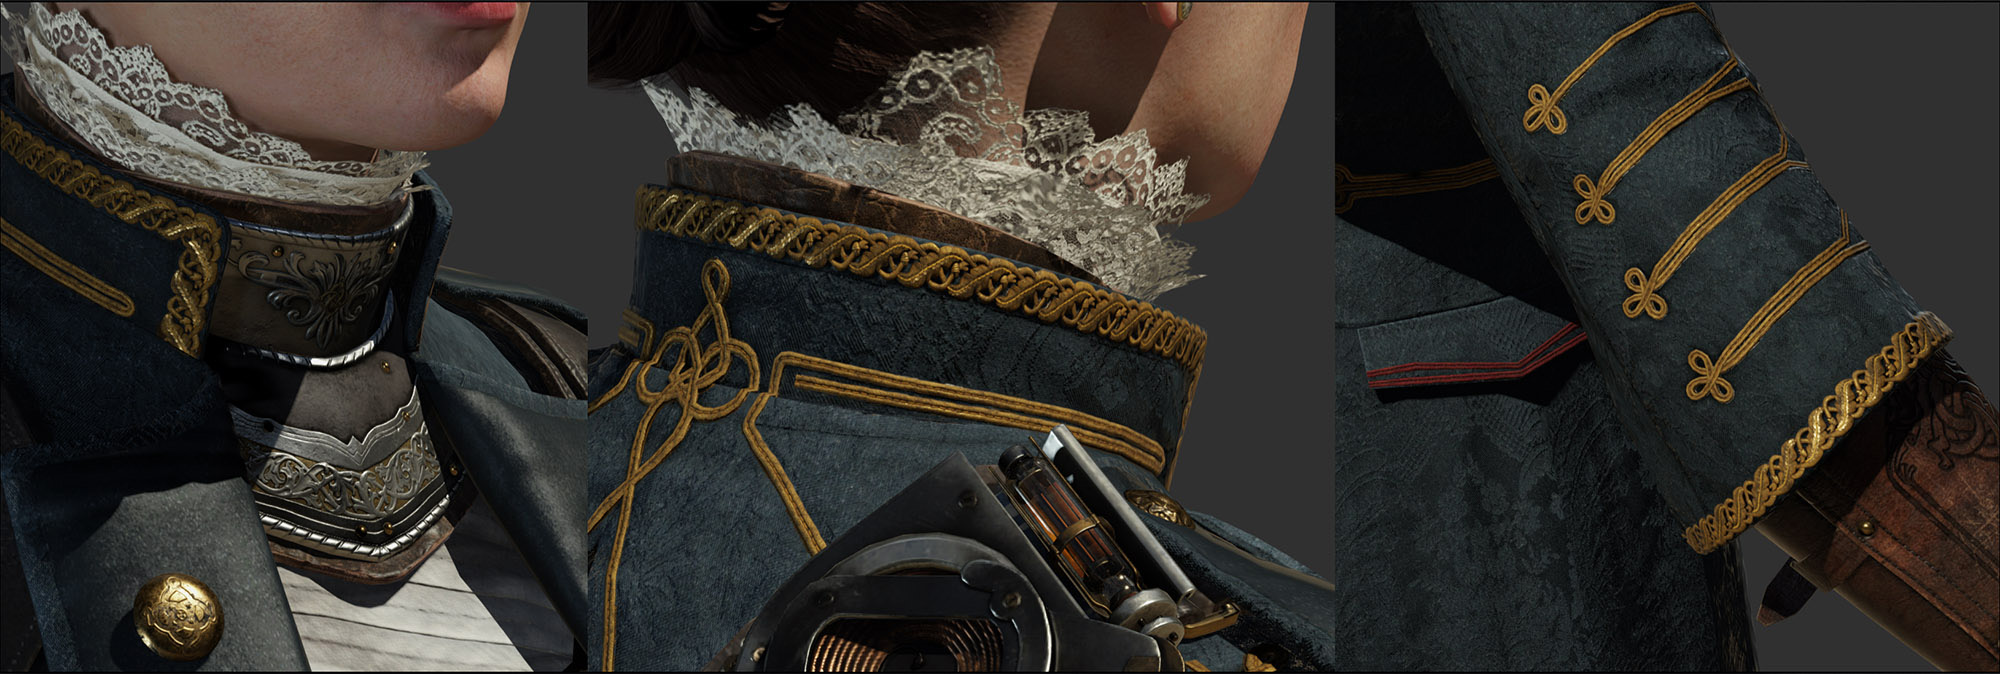
\includegraphics[scale=0.2]{theorder}}
    \caption{Im\'agenes del motor de renderizado hiperrealista en el videojuego The Order: 1886 \autocite{theorder}}
    \vspace{0.5cm}
\end{figure}

La intenci\'on de este proyecto es profundizar en las base te\'oricas de estas t\'ecnicas y aprender a integrarlas
dentro de un escenario real de trabajo, por lo que la colaboraci\'on con Seddi supone la ocasi\'on perfecta para la puesta en pr\'actica
de los conocimientos te\'oricos adquiridos.\\

La infraestructura de servicios en la nube sobre la que se sostiene Author me ha ofrecido la oportunidad de
aprender sobre la arquitectura, modelos de datos, sistemas de almacenamiento y protocolos de comunicaci\'on en sistemas distribu\'idos
en red. Por otra parte, la implementaci\'on de esta nueva funcionalidad en ThreeJs, la librer\'ia de 3D utilizada en Author,
me ha permitido entender como se integran estas t\'ecnicas dentro de la arquitectura de un motor de renderizado.\\

Adem\'as, como empleado de Seddi en el departamento de Author, entender mejor la infraestructura, el modelo de datos y las t\'ecnicas
de renderizado hiperrealistas que se utilizan en la empresa adem\'as de tratar de mejorar la experiencia de uso del contexto 3D de
la plataforma, son alicientes extra a las motivaciones citadas anteriormente.

\section{Objetivos}

La finalidad de este trabajo es proporcionar un nuevo modelo de material al contexto 3D de Author que represente mejor las propiedades
\'opticas de los tejidos y sea m\'as coherente con las im\'agenes de referencia generadas por un motor de trazado de rayos. Para la
consecuci\'on de esta tarea se trazan los siguientes objetivos generales:

\begin{enumerate}[label=(\roman*)]
	\item Dar soporte al nuevo material bajo la infraestructura de servicios en la nube de Seddi.
  \item Extender la librer\'ia ThreeJs para integrar un material espec\'ifico para la reproducci\'on de tejidos basado
  en aspectos f\'isicos o \textit{Physcally Based Rendering} (PBR).
\end{enumerate}

Que se componen de una serie de objetivos espec\'ificos:

\begin{enumerate}[label=\arabic*)]
	\item Adquirir conocimiento te\'orico sobre los motores de renderizado basados en aspectos f\'isicos.
    \item Adquirir conocimiento te\'orico sobre diferentes modelos de reflectancia o\\
    \textit{Bidirectional Reflectance Distribution Functions} (BRDFs)
    y sistemas de iluminaci\'on global en entornos interactivos de visualizaci\'on hiperrealista.
    \item Definici\'on del modelo para dar soporte al nuevo material dentro de la arquitectura de servicios en
    la nube de Seddi.
	\item Desarrollo de la interfaz de servicios en la nube para ofrecer soporte a este material.
	\item Entender a bajo nivel los detalles de implementaci\'on del sistema de renderizado de ThreeJs.
  \item Extender ThreeJs para integrar en su librer\'ia de materiales nativos el nuevo modelo de material orientado
  a la reproducci\'on de tejidos.
	\item Integrar el c\'odigo GLSL dentro del sistema de renderizado de ThreeJs para dar soporte al modelo de BRDF
	utilizado por el nuevo material.
\end{enumerate}

% Los principales objetivos del proyecto son crear un sistema para extender la librer\'ia de materiales de ThreeJs y a\~nadir a esta
% librer\'ia un nuevo material para ciertos tipos de tejidos basado en el modelo de BRDF para tejidos presentado por Filament. Estos
% objetivos generales se componen de una serie de objetivos espec\'ificos: entender la arquitectura del motor de renderizado de ThreeJs,
% los modelos de BRDF y sus implementaciones de materiales PBR de la librer\'ia est\'andar de ThreeJs y el modelo para tejidos de
% Filament, entender y ampliar el modelo de datos que representa los materiales en los servicios de Seddi, actualizar las interfaces
% que exponen la funcionanlidad sobre estos materiales y demostrar resultados en los que se aprecien los beneficies de utilizar este
% nuevo material frente a los materiales est\'andar de ThreeJs.

\section{Gu\'ia de la memoria}

\textbf{Cap\'itulo 1. Introducci\'on}
En este cap\'itulo se explican brevemente los objetivos y motivaciones del proyecto, as\'i como las aportaciones
de este trabajo.\\

\textbf{Cap\'itulo 2. Estado del arte}
El segundo cap\'itulo ofrece una visi\'on del estado del arte en cuanto a los trabajos sobre materiales e iluminaci\'on en tiempo real que guardan relaci\'on con la
soluci\'on presentada en este proyecto.\\

\textbf{Cap\'itulo 3. PBR}
En este cap\'itulo se explican las t\'ecnicas est\'andar en la actualidad para la representaci\'on de materiales realistas y
sirve como base te\'orica para los desarrollos presentados en los cap\'itulos 4 y 5.\\

\textbf{Cap\'itulo 4. Infraestructura y servicios web}
El cap\'itulo 4 explica la integraci\'on de la propuesta sobre los servicios en la nube de Seddi y la integraci\'on de un nuevo material
sobre la librer\'ia de WebgGL ThreeJs.\\

\textbf{Cap\'itulo 5. Modelos de iluminaci\'on para tejidos}
En este cap\'itulo se explica en detalle el modelo de BRDF a integrar para el material de tejidos y su implementaci\'on en ThreeJs.
Adem\'as se presentan resultados en los que se demuestran los nuevos efectos modelados por el material, as\'i como comparativas
del material est\'andar PBR de la librer\'ia frente al nuevo.\\

\textbf{Cap\'itulo 6. Discusi\'on y trabajo futuro}
Comentarios sobre el planteamiento, desarrollo, resultados obtenidos y posibles aplicaciones. Tambi\'en se establecen
l\'ineas de trabajo futuro.
